\documentclass[CJK]{beamer}
\usepackage{CJKutf8}
\usepackage{xcolor}
\usepackage{listings}
\usepackage{hyperref}
\hypersetup{
  urlcolor=blue,
  colorlinks=true,
  linkcolor=blue,
  bookmarks=false,
}
\usetheme{Boadilla}
\setbeamercovered{transparent}

\AtBeginSection[]
{
    \begin{frame}
        \tableofcontents[currentsection,hideallsubsections]
    \end{frame}
}
\AtBeginSubsection[]
{
    \begin{frame}[shrink]
        \tableofcontents[sectionstyle=show/shaded,subsectionstyle=show/shaded/hide]
    \end{frame}
}

\begin{document}
\begin{CJK*}{UTF8}{gbsn}

\title{且行且珍惜}
\subtitle{一年工作回顾}
\author{夏永锋}
\date{\today}

\begin{frame}
\titlepage
\end{frame}

\section*{大纲}
\begin{frame}
\tableofcontents
\end{frame}

\section{ECC电商运维平台}

\subsection{运营管理-易迅服务器视图}

\begin{frame}{服务器指标数据}
	\begin{block}{几点改进}
	\begin{itemize}
	\item 服务器分组排序展示
	\item 可灵活选择服务器
	\item 异步指标数据请求、数据加载提示、数据图绘制
	\item 数据图定期自动更新
	\end{itemize}
	\end{block}
\end{frame}

\begin{frame}{服务器归类视图}
	\begin{block}{功能点}
	\begin{itemize}
	\item 增、删、改、查服务器分类(树)
	\item 为服务器指定分类
	\item 服务器分类树数据可视化
	\item 强交互的服务器分类查询
	\end{itemize}
	\end{block}
	
	\begin{block}{难点}
	由manytoone(服务器$\rightarrow$分类)的关系数据构造出整个分类树,并且分类层次不限定。
	\end{block}
\end{frame}

\begin{frame}{服务器信息配置}
	\begin{block}{功能点}
	\begin{itemize}
	\item 服务器信息的增删改查
	\item 服务器告警屏蔽
	\end{itemize}
	\end{block}
	
	\begin{block}{亮点}
	\begin{itemize}
	\item 所有功能均以异步方式实现,无需页面跳转,体验与native app相近
	\item 告警屏蔽时间段可添加任意数量,并且对时间段进行排序和逻辑检测
	\end{itemize}
	\end{block}
\end{frame}

\begin{frame}{补充说明}
	\begin{itemize}
	\item 这三项功能是服务器监控的基础
	\item “服务器指标数据”依赖于“服务器信息配置”和“服务器归类视图”。若“服务器信息配置”中没有某服务器,那么即使该服务器上报了数据,在“服务器指标数据”中也查不到。若没有通过“服务器归类视图”归类某服务器,则该服务器在“服务器指标数据”中被归类到其他
	\end{itemize}
\end{frame}

\subsection{运营管理-易迅VIDC}

\begin{frame}{VIDC链路设备状态}
	\begin{block}{功能逻辑}
	\begin{enumerate}
	\item 用户在页面上通过“通道路由”或“最终目的”的ip和port查找相关的VIDC链路
	\item 后端代码在接收到AJAX请求后,获取请求参数,调用VIDC链路平台提供的API,得到链路结果后,
	对每条链路中涉及的机器ip进行分析(确定是腾讯IDC的还是易迅IDC的机器),并在返回的页面元素上打上标记
	\item 用户收到搜索结果后,点击某机器的ip,前端JS代码根据标记,向sh.ecc.com或TNM2上请求指标(CPU使用率和网卡的出/入流量)数据,并在页面上绘制数据图
	\end{enumerate}
	\end{block}
\end{frame}

\subsection{告警管理-页面监控}

\begin{frame}{应用场景}
\begin{block}{}
	大型web系统通常都有一个“统一接入层”,可以基于nginx实现,nginx根据HTTP请求头HOST字段的不同值,将请求转发到不同的后端机器集群(upstream)。
	
	基于URL的监控方案,如果仅是简单地直接访问页面,获取状态结果,只能证明当前站点服务还正常,但并不能证明每台后端机器都是正常工作的。所以若想定期地检测所有后端机器是否正常提供服务,则需要绕过“统一接入层”。
\end{block}
\end{frame}

\begin{frame}{方案}
\begin{block}{}
\begin{enumerate}
\item cron任务定期通过SSH获取“统一接入层”Nginx的配置,以正则表达式或状态机的方式解析配置,得到每个HOST对应哪个upstream,包含哪些后端机器,将数据存入数据库;
\item 另一个cron任务定期根据用户提供的需要监控的页面URL,取出该URL中的域名,根据该域名获取对应upstream的名称,根据该upstream的名称获取对应的机器列表,然后逐个机器地使用该机器ip(包括port)替换URL的域名部分,将域名放入HTTP请求头的HOST字段,发出请求,如果请求失败,则发送告警,并记录日志。
\end{enumerate}
\end{block}
\end{frame}

\begin{frame}{局限}
\begin{block}{}
由于Nginx的配置非常灵活,特别是如果Nginx在转发请求到后端机器之前改变了请求头的HOST字段的值,那么配置解析就很难获得正确的“HOST$\rightarrow$upstream$\rightarrow$后端机器列表”对应关系。
\end{block}
\end{frame}

\begin{frame}{易迅服务器Nginx配置}
\begin{block}{功能简介}
\begin{itemize}
\item 展示Nginx配置解析的结果
\item 提示用户Nginx配置变更情况
\item 提供Nginx配置的变更历史(粗粒度的版本控制)
\item 记录已删除掉的upstream
\item 人工维护对应到每个upstream的域名列表
\end{itemize}
\end{block}

\begin{block}{问题}
当域名和upstream数目很大时,人工维护“域名$\rightarrow$upstream”对应关系的工作量很大。但由于Nginx配置很灵活,很难自动解析得到该对应关系。
\end{block}

\end{frame}

\begin{frame}{易迅服务器curl监控}
\begin{block}{功能简介}
\begin{itemize}
\item 增、删、改、查监控项
\item 查看监控日志
\item 显示每个监控项最新检测的结果、错误数目。
\end{itemize}
\end{block}
\end{frame}

\subsection{系统管理-内容编辑}

\begin{frame}{新功能上线提示}
\begin{block}{动机}
每次新功能上线,都需要邮件周知,还不一定能周知到所有相关人,即使发送了,邮件也可能淹没在邮件的海洋中,或者很快就被接收人忘记。那么如何将开发人员从该问题中解脱出来?
\end{block}
\begin{block}{功能逻辑}
\begin{enumerate}
\item 开发人员在上线新功能后,在后台提交“新功能的URL”、“新功能简述”、“目标同事(腾讯、易迅)”等新功能信息
\item 系统登陆页面会在某个时间段内向用户显示后台提交的新功能上线提示信息
\end{enumerate}
\end{block}
\end{frame}

\section{运营开发规范化}
\begin{frame}{运营开发规范化}
\begin{itemize}
\item 详细说明见:\href{http://youngsterxyf.github.io/2013/10/15/standardization-operation-development/}{运营开发规范化}
\end{itemize}
\end{frame}

\section{高可用容灾方案}

\subsection{HAProxy + Keepalived}

\begin{frame}{系统架构图}
\begin{center}
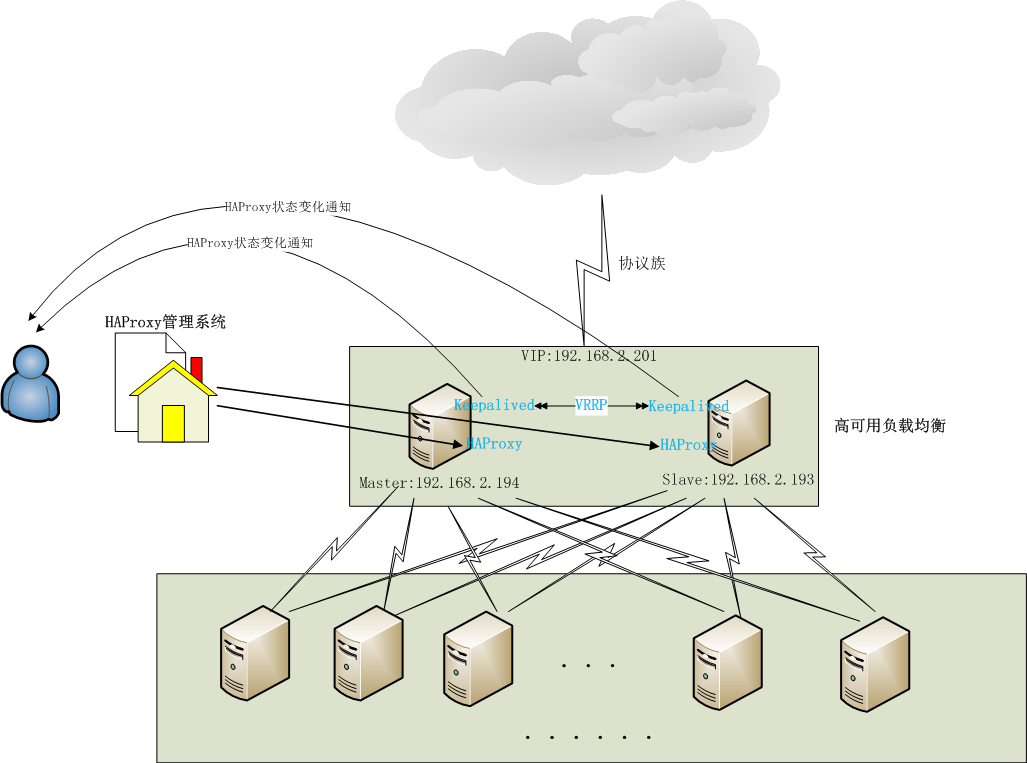
\includegraphics[height=8cm]{high-availability-load-balancer.png}
\end{center}
\end{frame}

\begin{frame}{HAProxy}

官网:\href{http://haproxy.1wt.eu/}{haproxy.1wt.eu}\\

\begin{itemize}
\item HAProxy是一款高性能的软件负载均衡器,提供4层\\(TCP)、7层(HTTP)协议代理
\item 在我们的应用中仅使用基于4层(TCP)协议的负载均衡
\end{itemize}
\end{frame}

\begin{frame}{Keepalived}
官网:\href{http://www.keepalived.org/}{www.keepalived.org}

\begin{block}{}
Keepalived是一个基于VRRP协议来实现的WEB服务高可用方案,可以利用其来避免单点故障。一个WEB服务至少会有2台服务器运行\\Keepalived,一台为主服务器(MASTER),一台为备份服务器\\(BACKUP),但是对外表现为一个虚拟IP,主服务器会发送特定的消息给备份服务器,当备份服务器收不到这个消息的时候,即主服务器宕机的时候,备份服务器就会接管虚拟IP,继续提供服务,从而保证了高可用性。
\end{block}
\begin{block}{}
Keepalived会定期检测HAProxy进程,如果主服务器的HAProxy进程挂掉,则Keepalived也会发生主从切换,在切换的时候会触发一个Python\\脚本(需自己实现)来发送邮件告警。
\end{block}
\end{frame}

\subsection{HAProxyConsole}
\begin{frame}{简介}
HAProxyConsole是一个自主开发的HAProxy负载均衡任务管理系统,能够极大地减轻运维人员的工作。
\begin{block}{相关材料}
\begin{itemize}
\item \href{http://youngsterxyf.github.io/2013/12/02/re_introduce_haproxyconsole/}{HAProxyConsole简介}
\item \href{http://pub.code.oa.com/project/home?projectName=HAProxyConsole}{公司公共组件页面}
\item \href{http://km.oa.com/group/geek/articles/show/172179}{公司内部推荐文章}
\item \href{https://github.com/youngsterxyf/haproxyconsole}{Github项目页面}
\end{itemize}
\end{block}
\end{frame}
\begin{frame}{系统原理图}
\begin{center}
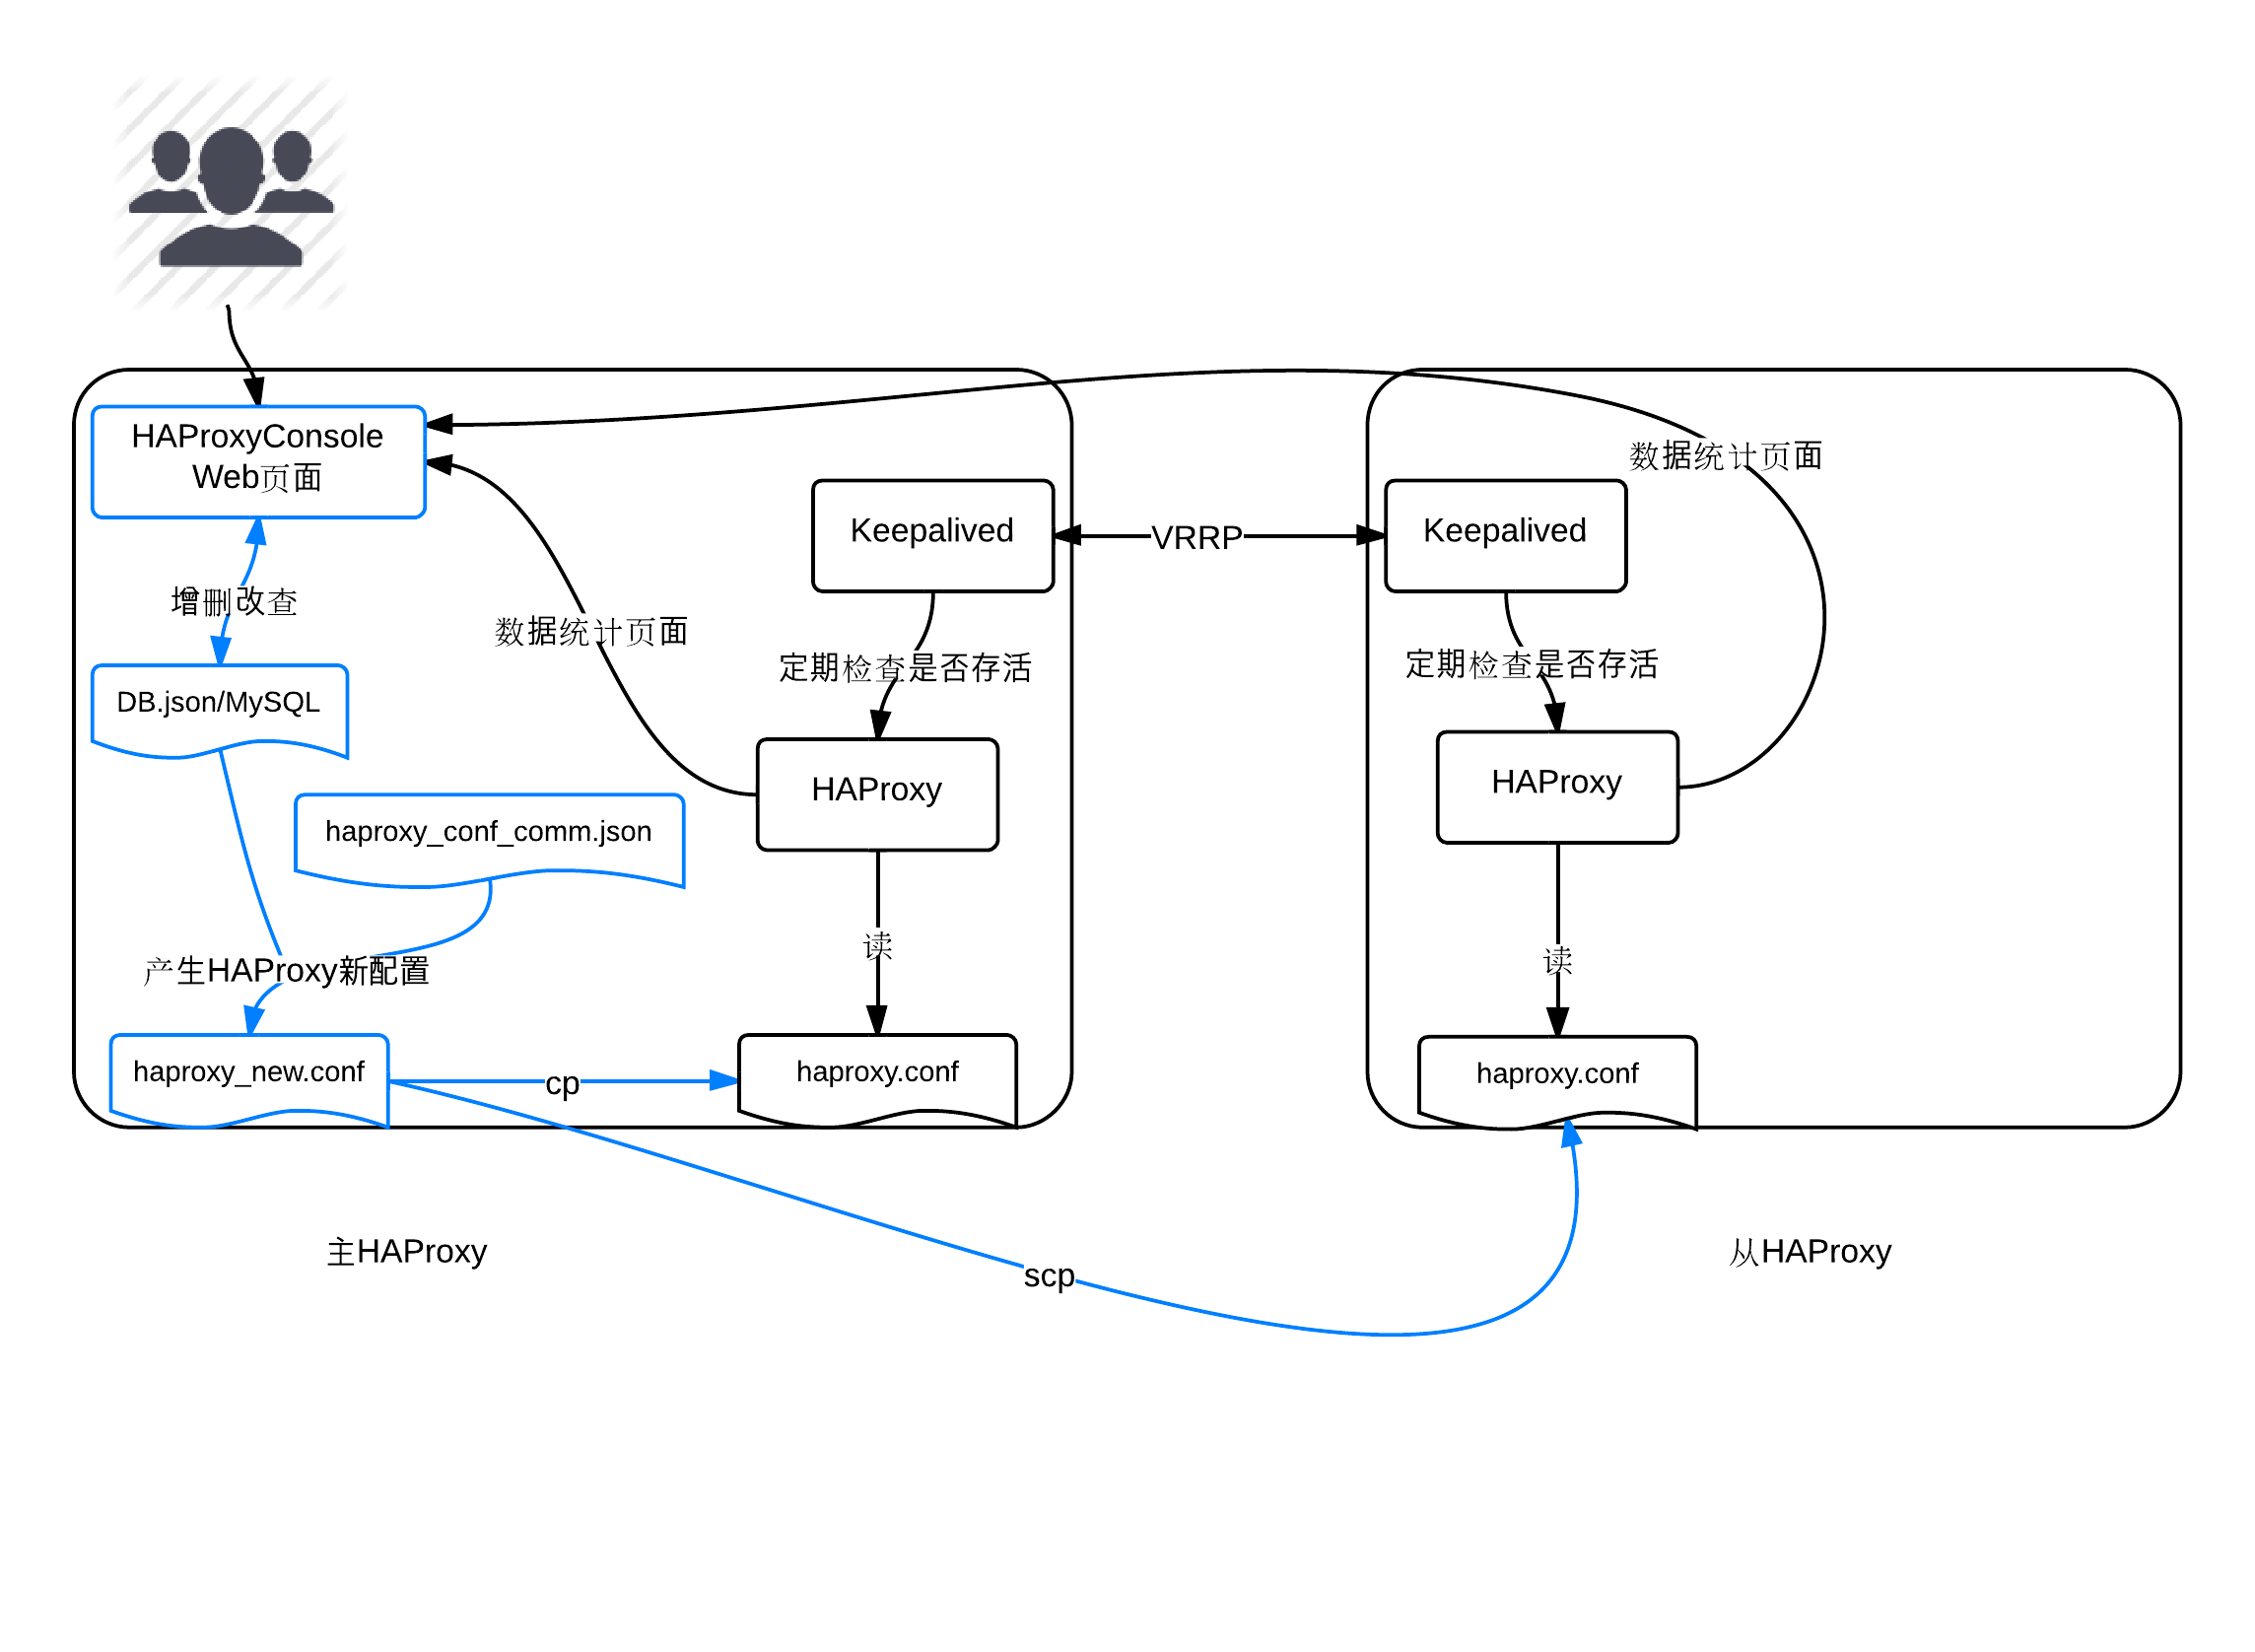
\includegraphics[height=8cm]{HAProxyConsole-arch.png}
\end{center}
\end{frame}

\subsection{缓存DNS}
\begin{frame}{缓存DNS}
\begin{itemize}
\item 采用BIND最新版本
\item 加速仓库机器DNS解析过程
\item 特定域名劫持
\item 不同网络提供商DNS服务容灾
\end{itemize}
\end{frame}

\subsection{自动化打包部署}
\begin{frame}[containsverbatim]{自动化打包部署}
\begin{itemize}
\item 针对仓库本地服务器编译打包,打包好的文件及脚本见\href{http://10.24.178.60:8000/yongfengxia/deploy_packages}{Gitlab代码仓库}。
\item \href{run:HAProxy_HAProxyConsole_Keepalived_BIND_Installation.pdf}{HAProxy+HAProxyConsole+Keepalived、BIND安装配置文档}
\item 此外,服务器192.168.2.193的/root/patch目录中有一组补丁(主要是服务的开机启动脚本)。在部署完成后,需将该目录远程拷贝到目标服务器,执行其中的patch.sh脚本即可(执行\verb"./patch.sh master"或\verb"./patch.sh slave")
\end{itemize}
\end{frame}

\section{仓库作业机器监控系统}

\subsection{仓库本地数据收集系统}

\begin{frame}{系统架构图}
\begin{center}
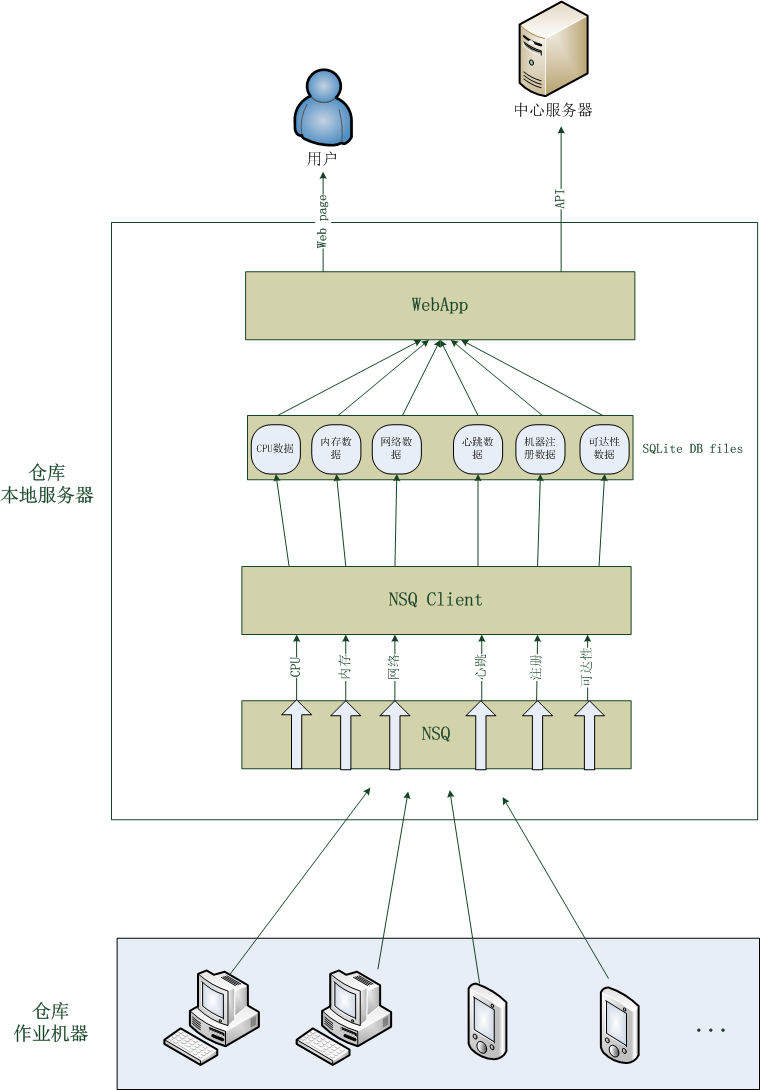
\includegraphics[height=10cm, angle=90]{inner_warehouse_monitor-arch.png}
\end{center}
\end{frame}

\begin{frame}{文档与代码}
\begin{itemize}
\item 文档见:\href{http://youngsterxyf.github.io/2013/11/29/inner_warehouse_monitor_system/}{仓库作业机器监控系统设计与实现}
\item 代码见:\href{http://10.24.178.60:8000/inner-warehouse-monitor}{inner-warehouse-monitor}
\end{itemize}
\end{frame}

\begin{frame}{消息队列-NSQ}
\begin{block}{为什么要使用消息队列?}
系统解耦。进入系统的数据量波动,不会影响系统的正常使用。
\end{block}
\begin{block}{NSQ的特性}
\begin{itemize}
\item 分布式、高性能
\item Go语言实现,静态编译,没有依赖,部署配置简单
\item 具备对用户透明的数据持久化
\item 内置管理统计功能
\item 已有成熟的生产应用
\end{itemize}
\end{block}
\end{frame}

\begin{frame}{数据存储方案}
\begin{block}{应用场景}
\begin{itemize}
\item 为了减少数据的网络传输量,每个仓库的监控数据都存储在仓库本地服务器上
\item 服务器的监控数据并不是强关系的数据,而是一种时间序列相关的数据,使用传统关系型数据来存储,反而会影响性能。
\item 对于多地部署的应用系统,使用独立的数据存储服务(如MySQL),运维成本较高。
\end{itemize}
\end{block}
\begin{block}{方案}
\begin{itemize}
\item 当前方案:使用SQLite,按“日期”、“机器IP”、“指标名称”进行分库
\item 备选方案1:使用时间序列数据库,如InfluxDB
\item 备选方案2:基于RRDtool
\end{itemize}
\end{block}
\end{frame}

\begin{frame}{数据展示平台}
\begin{itemize}
\item 前端实现:Bootstrap、jQuery、HighCharts、RaphaelJS等
\item 后端实现:Go语言Web框架Beego
\end{itemize}
\end{frame}

\subsection{统一平台}
\begin{frame}{统一平台网络架构}
\begin{center}
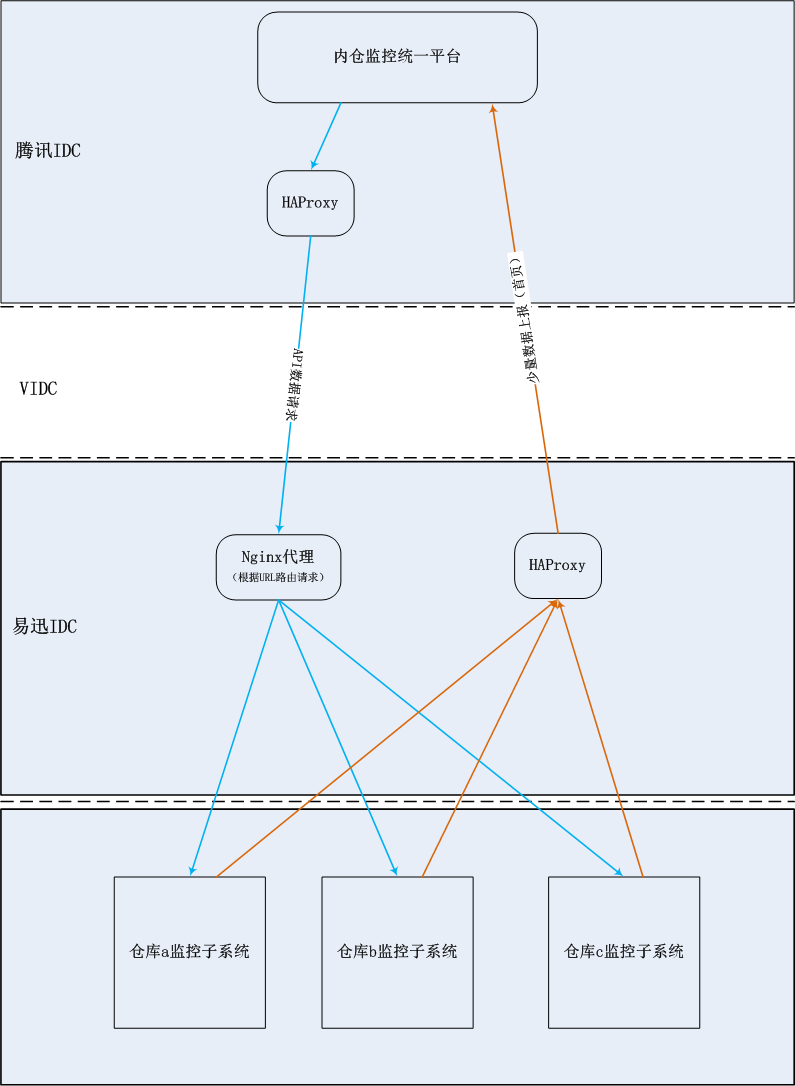
\includegraphics[height=8cm]{union-platform.png}
\end{center}
\end{frame}

\section{主要运维工作}
\begin{frame}{运维工作相关系统逻辑图}
\begin{center}
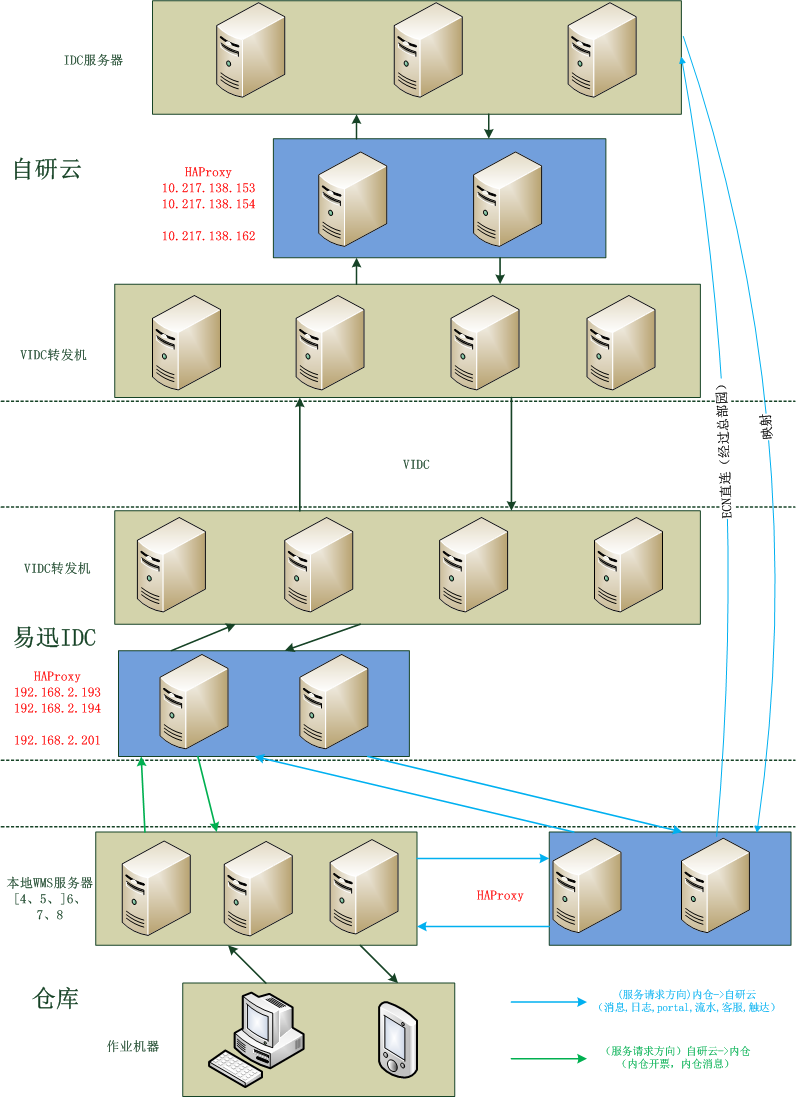
\includegraphics[height=10cm, angle=90]{iWMS.png}
\end{center}
\end{frame}

\section{其他}
\begin{frame}{WMS日志分析以及日报}
代码见:\href{http://10.24.178.60:8000/yongfengxia/wms_log_analysis}{wms\_log\_analysis}
\begin{itemize}
\item WMS日志数据存储在Windows服务器的SQL Server数据库中
\item Linux系统上cron任务通过FreeTDS协议远程查询所需数据,对获取到的数据统计分析后,通过公司的TOF API发送邮件日报
\end{itemize}
\begin{block}{难点}
FreeTDS库的编译安装、配置
\end{block}
\end{frame}

\begin{frame}{Nginx ip白名单增添服务}
代码见:\href{http://10.24.178.60:8000/yongfengxia/whitelistlistener}{WhiteListListener}
\begin{itemize}
\item 提供一个HTTP接口,用于在Nginx的ip白名单配置文件中添加新的ip
\item 具备基本的条件、安全检测
\end{itemize}
\end{frame}

\begin{frame}{VIDC链路检测告警}

代码见:\href{http://10.24.178.60:8000/yongfengxia/scripts/tree/master/vidcAlarm}{vidcAlarm}

\begin{block}{功能逻辑}
\begin{itemize}
\item cron任务脚本定期通过VIDC平台提供的API,获取解析链路数据,并直接检测每条链路的连通情况,当前正常的链路存入一个JSON\\文件中,也即将不连通的VIDC链路过滤掉
\item 另一个cron任务定期(如每3分钟)根据前一个cron任务产生的JSON文件,逐一检测VIDC链路,若某链路不通,但前一次检测是通的,则发送链路异常告警,并将该链路记录下来; 若当前检测链路正常,但前一次检测是不通的,则发送链路恢复告警,并从异常链路记录中删除该链路。
\end{itemize}
\end{block}
\begin{block}{亮点}
通过协程的方式来并发检测链路,相比之前串行的检测方式,效率提高了几十倍,当然实现逻辑更复杂了点。
\end{block}
\end{frame}
\end{CJK*}
\end{document}
